\subsection{Data Memory}
\begin{figure}[!ht]
    \centering
    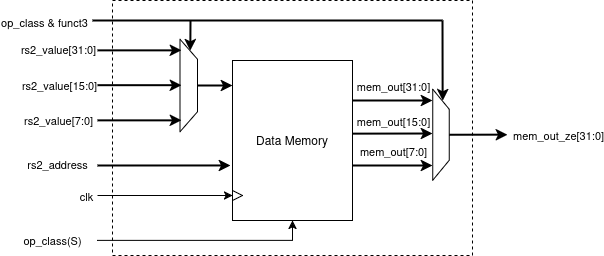
\includegraphics[scale = 0.45]{MEM_BD.png}
    \caption{DM interface block diagram}
    \label{fig:DM_BD}
\end{figure}

The final pieces that are left to be designed are the one that manage the Data Memory, the one which decides when to write and where, and the stage which, depending on the operation type, selects what to return as new value for the PC and what to store in the destination register, i.e the Write Back.\\
The Data Memory will instantiated as a 16KB single port RAM and separated from the rest, forming a 5-stage datapath when it is going to be pipelined. In 4-stages architecture it would be instead included in the same block, reducing the overall size of the processor, reducing power consumption, due to the presence of one less register, but at the cost of a reduced throughput.\\
The Table \ref{table:core_instr} indicates that there are many ways to perform L/S instruction and not only 32-bit vectors are handled. In fact some of them could manage just bytes or half-words, leaving some other options to be managed when executing these instructions. This discrimination cannot be performed by the ALU nor the Decoder, but it is easy to implement as interface for the Data Memory.
To be more specific, another case statement can be deployed to select filter the input and output of and from the memory, leaving the discrimination to both \emph{op{\_}class}, to see if an L/S operation is being performed, and \emph{funct3} to classify if the latter is working with bytes, half-words or words.

\subsection{Write Back}
\begin{figure}[!ht]
    \centering
    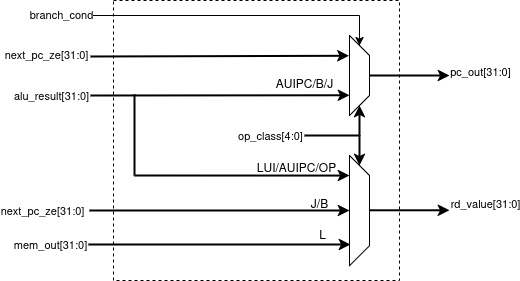
\includegraphics[scale = 0.45]{WB_BD.png}
    \caption{Write Back block diagram}
    \label{fig:WB_BD}
\end{figure}

The final step of execution, where the destination register and the program counter are written, needs a selector to decide what has to be overwritten and where; In the case of the PC two options can be identified: PC + 4 or the result from the ALU, which happens in case of a jump, a true condition from a branch or AUIPC. The destination register instead can be: the output of the ALU for classes OP, LUI, UIPC, PC + 4 for jumps and branches (when a logic high is returned, otherwise a high impedance output can be returned) or the output from the data memory. Source Code \ref{code:WB_code} shows again a case statement enclosed in an input-sensitive process, that is, a simple combinatory network.\\
The reading and writing of the register file in the same clock cycle might seem impossible, since \emph{rs1} would have to be selected before the execution happens, meaning it  

\subsection{Simulation and final consideration}
With all the code prepared, the final simulation of the unpipelined datapath can be performed; Leaving the load-enable of the PC high, for there is no need to stall the execution for now, it is noticeable that the overall behavior corresponds to what is expected from it:

\begin{figure}[!ht]
    \centering
    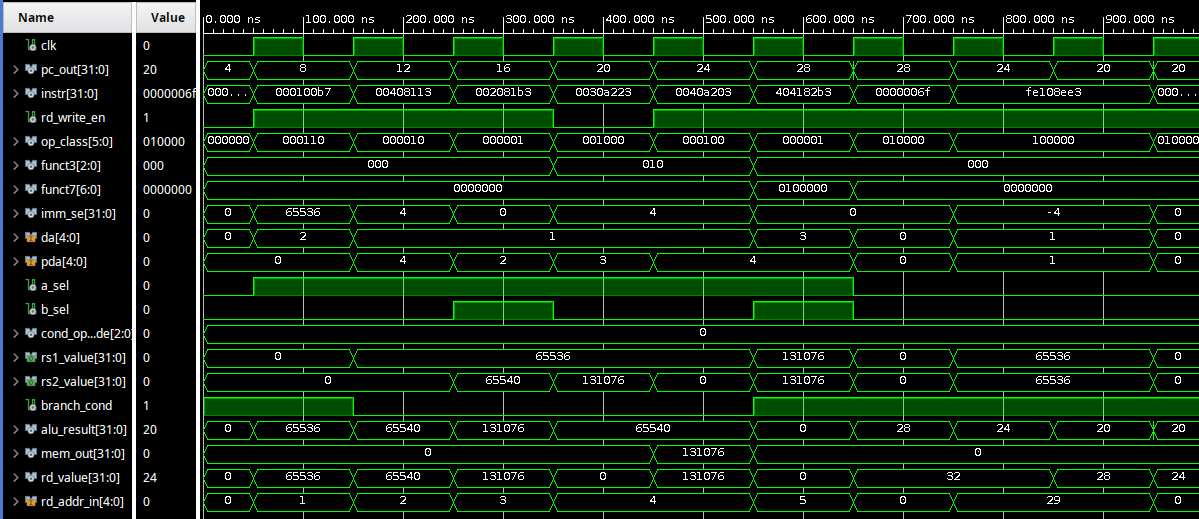
\includegraphics[scale = 0.36]{WB_sim.png}
    \caption{Complete simulation of the unpipelined datapath}
    \label{fig:WB_sim}
\end{figure}

Jumps and branches seem to be able to actively change the PC, in fact, the branch returns the value of PC where the sub instruction is located, meaning that if the simulation were to run infinitely, the program would loop between PC=28 and PC=32.\\ 
Also it is noticeable that L/S operations can effectively interact with the memory, although not each one of them has been tested, and other instruction can successfully read and write from the register file.